% !TEX root = collection.tex

\subsection{PRG Extension}
In this section we show that any pseudorandom generator that produces one bit of randomness can be extended to create a polynomial number of bits of randomness.

\begin{construction}
Given a PRG $G: \{0, 1\}^n \rightarrow \{0, 1\} ^ {n+1}$,
we construct a new PRG $F: \{0, 1\}^n \rightarrow \{0, 1\} ^{n+l}$ as follows ($l$ is polynomial in $n$).
\begin{enumerate}[label=(\alph*)]
    \item Input: $S_0 \xleftarrow{\$} \{0, 1\}^n$.
    \item $\forall i \in [l] = \{1, 2, \cdots, l\}$, $(\sigma_i, S_i) := G(S_{i-1})$, where $\sigma_i \in \{0, 1\}, S_i \in \{0, 1\}^n$ .
    \item Output: $\sigma_1 \sigma_2 \cdots \sigma_l S_l$.
\end{enumerate}
\end{construction}

\begin{theorem}
The function $F$ constructed above is a PRG.
\end{theorem}

\proof
We prove this by hybrid argument. Define the hybrid $H_i$ as follows.
\begin{enumerate}[label=(\alph*)]
	\item Input: $S_0 \xleftarrow{\$} \{0, 1\}^n$.
    \item $\sigma_1, \sigma_2, \cdots, \sigma_i \xleftarrow{\$} \{0, 1\}$, $S_i \gets S_0$.\\
     $\forall j \in \{i+1, i+2, \cdots, l\}$, $(\sigma_j, S_j) := G(S_{j-1})$, where $\sigma_j \in \{0, 1\}, S_j \in \{0, 1\}^n$ .
    \item Output: $\sigma_1 \sigma_2 \cdots \sigma_l S_l$.
\end{enumerate}
Note that $H_0 \equiv F$, and $H_l \equiv U_{n+l}$.

Assume for the sake of contradiction that there exits a non-uniform PPT adversary $\ma$ that can distinguish $H_0$ form $H_l$.
Define $\epsilon_i := \Pr[\ma(1^n, H_i)=1]$ for $i = 0, 1, \cdots, l$.
Then there exists a non-negligible function $v(n)$ such that $|\epsilon_0 - \epsilon_l| \geq v(n)$.
Since
\[
|\epsilon_0 - \epsilon_1| +
|\epsilon_1 - \epsilon_2| +
\cdots +
|\epsilon_{l-1} - \epsilon_l| \geq
|\epsilon_0 - \epsilon_l|
\geq v(n),
\]
there exists $k \in \{0, 1, \cdots, l-1\}$ such that
\[
|\epsilon_{k} - \epsilon_{k+1}| \geq \frac{v(n)}{l}.
\]
$l$ is polynomial in $n$, hence $\frac{v(n)}{l}$ is also a non-negligible function.
That is to say, $\ma$ can distinguish $H_{k}$ from $H_{k+1}$.
Then we use $\ma$ to construct an adversary $\mathcal{B}$ that can distinguish $U_{n+1}$ from $G(U_n)$ (which leads to a contradiction):
On input $T \in \{0, 1\}^{n+1}$ ($T$ could be either from $U_{n+1}$ or $G(U_n)$), $\mathcal{B}$ proceeds as follows:
\begin{itemize}
\item $\sigma_1, \sigma_2, \cdots, \sigma_k \xleftarrow{\$} \{0, 1\}$, $(\sigma_{k+1}, S_{k+1}) \gets T$.
\item $\forall j \in \{k+2, k+3, \cdots, l\}$, $(\sigma_j, S_j) := G(S_{j-1})$, where $\sigma_j \in \{0, 1\}, S_j \in \{0, 1\}^n$ .
\item Output: $\ma(1^n, \sigma_1 \sigma_2 \cdots \sigma_l S_l)$.
\end{itemize}

First, since $\ma$ and $G$ are both PPT computable, $\mathcal{B}$ is also PPT computable.

Second, if $T\gets G(U_n)$, then $\sigma_1 \sigma_2 \cdots \sigma_l S_l$ is the output of  $H_{k}$; if $T \stackrel{\$}\leftarrow U_{n+1}$, then $\sigma_1 \sigma_2 \cdots \sigma_l S_l$ is the output of $H_{k+1}$.
Hence
\begin{align*}
&\big|\Pr[\mathcal{B}(1^n, G(U_n)) = 1] - \Pr[\mathcal{B}(1^n, U_{n+1}) = 1]\big|\\
=& \big|\Pr[\ma(1^n,H_k) = 1] - \Pr[\ma(1^n,H_{k+1}) = 1]\big|\\
=&
|\epsilon_{k} - \epsilon_{k+1}| \geq \frac{v(n)}{l}.
\end{align*}
\qed

\subsection{PRG from OWP (One-Way Permutations)}
In this section we show how to construct pseudorandom generators under the assumption that one-way permutations exist.

\begin{construction}
Let $f: \{0, 1\}^n \rightarrow \{0, 1\}^n$ be a OWP. We construct $G: \{0, 1\}^{2n} \rightarrow \{0, 1\}^{2n+1}$ as
\[
G(x, r) = f(x) || r || B(x, r),
\]
where $x, r \in \{0, 1\}^n$, and $B(x, r)$ is a hard core bit for the function $g(x,r) = f(x) || r$.
\end{construction}

\begin{remark}
The hard core bit $B(x,r)$ always exists. Recall Theorem~\ref{thm:hard-core-bit},
\[B(x,r) = \left(\sum_{i=1}^n x_i r_i\right)\mod 2\]
is a hard core bit.
\end{remark}

\begin{theorem}
The $G$ constructed above is a PRG.
\end{theorem}

\proof
Assume for the sake of contradiction that $G$ is not PRG.
We construct three ensembles of probability distributions:
\[H_0 := G(U_{2n}) = f(x) || r || B(x, r), \text{ where } x, r \xleftarrow{\$} \{0, 1\}^n;\]
\[H_1 := f(x) || r || \sigma, \text{ where } x, r \xleftarrow{\$} \{0, 1\}^n, \sigma \xleftarrow{\$} \{0, 1\};\]
\[H_2 := U_{2n+1}.\]

Since $G$ is not PRG, there exists a non-uniform PPT adversary $\ma$ that can distinguish $H_0$ from $H_2$.
Since $f$ is a permutation, $H_1$ is uniformly distributed in $\{0, 1\}^{2n+1}$, i.e., $H_1 \equiv H_2$.
Therefore, $\ma$ can distinguish $H_0$ from $H_1$,
that is, there exists a non-negligible function $v(n)$ satisfying
\[
\big| \Pr[\ma(H_0)=1] - \Pr[\ma(H_1)=1] \big| \geq v(n).
\]

Next we will construct an adversary $\mathcal{B}$ that ``breaks'' the hard core bit (which leads to a contradiction).
Define a new ensemble of probability distribution
\[
H_1' = f(x) || r || (1-B(x, r)) , \text{ where } x, r \xleftarrow{\$} \{0, 1\}^n.
\]
Then we have
\begin{align*}
\Pr[\ma(H_1) = 1]
=& \Pr[\sigma = B(x, r)] \Pr[A(H_0) = 1] + \Pr[\sigma = 1 - B(x, r)] \Pr[A(H_1') = 1]\\
=& \frac{1}{2} \Pr[A(H_0) = 1] + \frac{1}{2}\Pr[A(H_1') = 1].
\end{align*}
Hence
\begin{align*}
&\Pr[A(H_1) = 1] - \Pr[A(H_0) = 1]
=  \frac{1}{2}\Pr[A(H_1') = 1] - \frac{1}{2} \Pr[A(H_0) = 1],
\\
&\frac{1}{2} \left|\Pr[A(H_0) = 1] - \Pr[A(H_1') = 1] \right|
= \left| \Pr[A(H_1) = 1] - \Pr[A(H_0) = 1] \right|
\geq v(n),
\\
&\left|\Pr[A(H_0) = 1] - \Pr[A(H_1') = 1] \right|
\geq 2v(n).
\end{align*}

Without loss of generality, we assume that
\[
\Pr[A(H_0) = 1] - \Pr[A(H_1') = 1]
\geq 2v(n).
\]
Then we construct $\mathcal{B}$ as follows:
\[
\mathcal{B}(f(x)|| r) :=
\begin{cases}
\sigma, & \text{if } \ma(f(x)|| r||\sigma) = 1\\
1 - \sigma, & \text{if } \ma(f(x)||r|| \sigma) = 0
\end{cases},
\]
where $\sigma \xleftarrow{\$} \{0, 1\}$.
Then we have
\begin{align*}
& \Pr[\mathcal{B}(f(x)|| r) = B(x, r)]\\
=& \Pr[\sigma = B(x, r)] \Pr[ \ma(f(x)|| r||\sigma)=1 | \sigma = B(x, r)] + \\
& \Pr[\sigma = 1 - B(x, r)] \Pr[ \ma(f(x)|| r||\sigma) = 0 | \sigma = 1- B(x, r)] + \\
=& \frac{1}{2} \big( \Pr[\ma(f(x)||r||B(x, r)) = 1] + 1 - \Pr[\ma(f(x)|| r|| 1- B(x, r)) = 1] \big)\\
=& \frac{1}{2} + \frac{1}{2} \big( \Pr[A(H_0) = 1] - \Pr[A(H_1') = 1] \big)\\
\geq & \frac{1}{2} + v(n).
\end{align*}
Contradiction with the fact that $B$ is a hard core bit.
\qed

\section{Pseudorandom Functions}
In this section, we first define pseudorandom functions, and then show how to  construct a pseudorandom function from a pseudorandom generator.

Considering the set of all functions $f: \{0, 1\}^n \rightarrow \{0, 1\}^n$, there are $(2^n)^{2^n}$ of them.
To describe a random function in this set we need $n \cdot 2^n$ bits.
Intuitively, a pseudorandom function is one that cannot be distinguished from a random one,
but needs much fewer bits (e.g., polynomial in $n$) to be described.
Note that we restrict the distinguisher to only being allowed to ask the function poly($n$) times and decide whether it is random or pseudorandom.

\subsection{Definitions}

\begin{definition}[Function Ensemble]
A \emph{function ensemble} is a sequence of random variables $F_1, F_2, \cdots, F_n, \cdots$ denoted as $\{F_n\}_{n \in \mathbb{N}}$ such that
$F_n$ assumes values in the set of functions mapping $n$-bit input to $n$-bit output.
\end{definition}

\begin{definition}[Random Function Ensemble]
We denote a random function ensemble by $\{R_n\}_{n \in \mathbb{N}}$.
\end{definition}

\begin{definition}[Efficiently Computable Function Ensemble]
A function ensemble is called \emph{efficiently computable} if
\begin{enumerate}[label=(\alph*)]
    \item \textbf{Succinct}:
        $\exists$ a PPT algorithm $I$ and a mapping $\phi$ from strings to functions such that
        $\phi(I(1^n))$ and $F_n$ are identically distributed.
        Note that we can view $I$ as the description of the function.
    \item \textbf{Efficient}:
        $\exists$ a poly-time machine $V$ such that
        $V(i, x) = f_i(x)$ for every $x \in \{0, 1\}^n$, where $i$ is in the range of $I(1^n)$, and $f_i = \phi(i)$.
\end{enumerate}
\end{definition}

\begin{definition}[Pseudorandom Function Ensemble]
A function ensemble $F = \{F_n\}_{n \in \mathbb{N}}$ is \emph{pseudorandom} if
for every non-uniform PPT oracle adversary $\ma$, there exists a negligible function $\epsilon(n)$ such that
\[
\big| \Pr[\ma^{F_n} (1^n) = 1] - \Pr[\ma^{R_n} (1^n) = 1]  \big| \leq \epsilon(n).
\]
Here by saying ``oracle'' it means that $\ma$ has ``oracle access'' to a function (in our definition, the function is $F_n$ or $R_n$), and each call to that function costs 1 unit of time.
\end{definition}

Note that we will only consider efficiently computable pseudorandom ensembles in the following.

\subsection{Construction of PRF from PRG}

\begin{construction}
Given a PRG $G: \{0, 1\}^n \rightarrow \{0, 1\}^{2n}$,
let $G_0(x)$ be the first $n$ bits of $G(x)$, $G_1(x)$ be the last $n$ bits of $G(x)$.
We construct $F^{(K)}: \{0, 1\}^n \rightarrow \{0, 1\}^n$ as follows.
\[
F^{(K)}_n(x_1 x_2 \cdots x_n) := G_{x_n}(G_{x_{n-1}} (\cdots(G_{x_1}(K)) \cdots  )),
\]
where $K \in \{0,1\}^n$ is the key to the pseudorandom function. Here $i$ is an $n$-bit string, which is the seed of the pseudorandom function.
\end{construction}
The construction can be viewed as a binary tree of depth $n$, as shown in Figure \ref{fig:binary-tree}.

\begin{figure}[h]
    \centering
    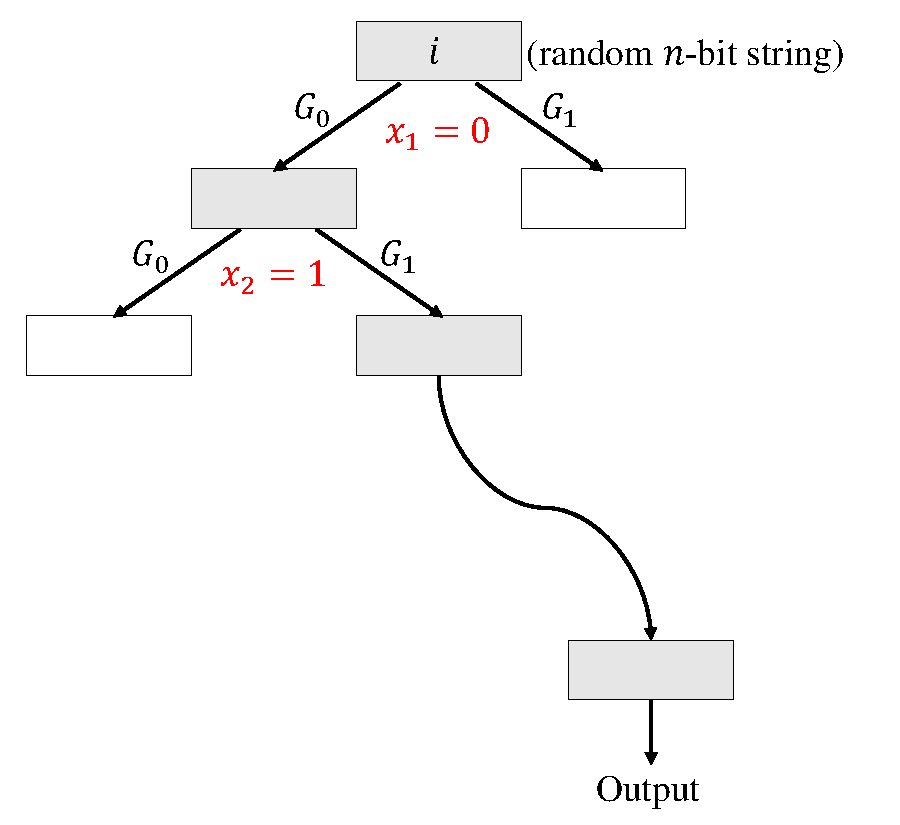
\includegraphics[width=0.5\textwidth]{binary-tree.pdf}
    \caption{View the construction as a binary tree}
    \label{fig:binary-tree}
\end{figure}

\begin{theorem}\label{theorem:ggm}
The function ensemble $\{F_n\}_{n \in \mathbb{N}}$ constructed above is pseudorandom.
\end{theorem}

\proof
Assume for the sake of contradiction that $\{F_n\}_{n \in \mathbb{N}}$ is not PRG.
Then there exists a non-uniform PPT oracle adversary $\ma$ that can distinguish $\{F_n\}_{n \in \mathbb{N}}$ from $\{R_n\}_{n \in \mathbb{N}}$. Below, via a hybrid argument, we prove that this contradicts the fact that $G$ is a PRG.

Consider the sequence of hybrids $H_i$ for $i \in \{ 0, 1, \cdots, n\}$ where the hybrid $i$ is defined as follows:
\[H_{n,i}^{(K)} (x_1x_2\ldots x_n ):= G_{x_n}(G_{x_{n-1}} (\cdots(G_{x_{i+1}}(K(x_ix_{i-1}\ldots x_1))) \cdots  )), \]
where $K$ is a random function from $\{0,1\}^{i}$ to $\{0,1\}^n$. Intuitively, hybrid $H_i$ corresponds to a binary tree of depth $n$ where the nodes of levels $0$ to $i$ correspond to random values and the nodes at levels $i+1$ to $n$ correspond to pseudorandom values. By inspection, observe that hybrids $H_0$ and $H_n$ are identical to a pseudorandom function and a random function, respectively. There it suffices to prove that hybrids $H_i$ and $H_{i+1}$ are computationally indistinguishable for each $i \in \{ 0, 1, \cdots, n\}$.

We show that $H_{i}$ and $H_{i+1}$ are indistinguishable by considering a sequence of sub-hybrids $H_{i,j}$ for $j \in \{0,\ldots q_{i+1}\}$, where $q_{i+1}$ is the number of the distinct $i-bit$ prefixes of the queries of $\mathcal{A}$.\footnote{Observe that $q_{i+1}$ for each appropriate choice of $i$ is bounded by the running time of $\mathcal{A}$. Hence, this value is bounded by a polynomial in the security parameter.}

We define hybrid $H_{i,j}$ for $j =0$ to be same as hybrid $H_{i}$. Additionally, for $j >0$ hybrid $H_{i,j}$ is defined to be exactly the same as hybrid $H_{i,j-1}$ except the response provided to the attacker for the $j^{th}$ distinct $i-bit$ prefix query of $\mathcal{A}$. Let this prefix be $x^*_n x^*_{n-1} \ldots x^*_{i}$. Note that in hybrid $H_{i,j-1}$ the children of the node $x^*_n x^*_{n-1} \ldots x^*_{i}$ correspond to two pseudorandom values. In hybrid $H_{i,j}$ we replace these two children with random values. By careful inspection, it follows that hybrid $H_{i,q_{i+1}}$ is actually $H_{i+1}$. All we are left to prove is that hybrid $H_{i,j}$ and $H_{i,j+1}$ are indistinguishable for the appropriate choices of $j$ and we prove this below.


Now we are ready to construct an adversary $\mathcal{B}$ that  distinguishes $U_{2n}$ from $G(U_n)$: On input $T \in\{0, 1\}^{2n}$ ($T$ could be either from $U_{2n}$ or $G(U_n)$),
construct a full binary tree of depth $n$ that is exactly the same as $H_{i,j}$ except replacing the children of  $x^*_n x^*_{n-1} \ldots x^*_{i}$ by the value $T$.
Observe that the only difference between $H_{i,j}$ and $H_{i,j+1}$ is that values corresponding to nodes $x_n^*\ldots x_i^* 0$ and $x_n^*\ldots x_i^* 1$ are pseudorandom or random respectively. $\mathcal{B}$ uses the value $T$ to generate these two nodes. Hence success in  distinguishing hybrids $H_{i,j}$ and $H_{i,j+1}$ provides a successful attack for $\mathcal{B}$ in violating security of the pseudorandom generator.
\qed

\section*{Exercises}
\begin{exercise}
\newcommand{\bit}{\{0,1\}}

Prove or disprove: If $f$ is a one-way function, then the following function $B:\bit^*\to\bit$ is a hardcore predicate for $f$. The function $B(x)$ outputs the inner product modulo 2 of the first $\lfloor |x|/2\rfloor$ bits of $x$ and the last $\lfloor |x|/2\rfloor$ bits of $x$.
\end{exercise}

\begin{exercise}
Let $\phi(n)$ denote the first $n$ digits of $\pi = 3.141592653589\ldots$ after the decimal in binary ($\pi$ in its binary notation looks like $11.00100100001111110110101010001000100001\ldots$).

   Prove the following: if one-way functions exist, then there exists a one-way function $f$ such that the function $B:\{0,1\}^* \rightarrow \{0,1\}$ is not a hard core bit of $f$. The function $B(x)$ outputs $\langle x, \phi(|x|)\rangle$, where
    \[\langle a, b\rangle := \sum_{i=1}^n a_i b_i \mod 2\]
    for the bit-representation of $a = {a_1a_2\cdots a_n}$ and $b= {b_1b_2\cdots b_n}$.
\end{exercise}

\begin{exercise}
 If $f: \{0,1\}^{n}\times \{0,1\}^n\rightarrow \{0,1\}^n$  is PRF, then in which of the following cases is $g: \{0,1\}^{n}\times \{0,1\}^n\rightarrow \{0,1\}^n$ also a PRF? \begin{enumerate} \item $g(K,x) = f(K,f(K,x))$ \item $g(K,x) = f(x,f(K,x))$ \item $g(K,x) = f(K,f(x,K))$
    \end{enumerate}
\end{exercise}

\begin{exercise}[Puncturable PRFs.] Puncturable PRFs are PRFs for which a key can be given out such that, it allows evaluation of the PRF on all inputs, except for one designated input.

\newcommand{\negl}{\mathsf{negl}}
\newcommand{\A}{\mathcal{A}}
\newcommand{\F}{F}
\newcommand{\KeyF}{\mathsf{Key}_{\F}}
\newcommand{\PunctureF}{\mathsf{Puncture}_{\F}}
\newcommand{\EvalF}{\mathsf{Eval}_{\F}}


A puncturable pseudo-random function $\F$ is given by a triple of efficient algorithms ($\KeyF$,$\PunctureF$, and $\EvalF$), satisfying the following conditions:
\begin{itemize}
\item[-] \textbf{Functionality preserved under puncturing}: For every $x^*, x \in \{0,1\}^{n}$ such that $x^* \neq x$, we have that:
    $$\Pr[\EvalF(K,x) = \EvalF(K_{x^*},x) : K \gets \KeyF(1^n), K_{x^*} = \PunctureF(K,x^*)] = 1$$
\item[-] \textbf{Pseudorandom at the punctured point}: For every $x^*\in \{0,1\}^n$ we have that for every polysize adversary $\A$ we have that:
    $$|\Pr[\A(K_{x^*}, \EvalF(K,x^*)) = 1] - \Pr[\A(K_{x^*}, \EvalF(K,U_n)) = 1]|= \negl(n)$$
    where $K \gets \KeyF(1^n)$ and $K_S = \PunctureF(K,x^*)$. $U_n$ denotes the uniform distribution over $n$ bits.
\end{itemize}

Prove that: If one-way functions exist, then there exists a puncturable PRF family that maps $n$ bits to $n$ bits. \\ \\
\textbf{Hint:} The GGM tree-based construction of PRFs from a length doubling pseudorandom generator (discussed in class) can be adapted to construct a puncturable PRF. Also note that $K$ and $K_{x^*}$ need not be the same length.
\end{exercise}
%
%\subsection{Application}
%Consider an interesting game: Alice and Bob are talking on the phone.
%Alice flips a coin, and Bob guesses whether it's head or tail.
%But the problem is how can Alice convince Bob that the coin is indeed head or tail?
%If we have pseudorandom functions, the problem could be easily solved.
%
%Assume we have a PRF $F_n: \{0, 1\}^n \rightarrow \{0, 1\}^n$.
%Alice and Bob have a shared key $i \in \{0, 1\}^n$, then $f_i(\cdot)$ is shared information.
%Now Alice has a message $m \in \{0, 1\}^n$ and wants to let Bob guess it,
%the procedure consists of three steps.
%\begin{enumerate}[(a)]
%    \item Alice chooses a string $r \in \{0, 1\}^n$, and sends to Bob  $m' = f_i(r) \oplus m$ ;
%    \item Bob guesses $m$;
%    \item Alice sends $r$ to Bob.
%\end{enumerate}
%In step (a), since $F_n$ is PRF, all the information that Bob gets is a random $n$-bit string, so it will not influence his behavior in step (b).
%Then in step (c), Bob receives $r$ and will be convinced that the true value of $m$ is $f_i(r) \oplus m'$.
%
%
